% !TeX encoding = UTF-8
% !TeX program = xelatex
% !TeX spellcheck = en_US

% XMU Thesis LaTeX template

\documentclass{xmuthesis}

\xmusetup{
  % 论文(设计)标题
  title = 面向非结构化企业指标信息的智能处理和可视分析,
  % 论文(设计)英文标题
  en-title = Indicators of the Unstructured Information for Intelligence Processing and Visualization,
  % 作者
  author = 王嘉然,
  % 学号
  student-no = 1145141919810,
  % 学院
  institute = 信息学院,
  % 专业
  profession = 计算机科学与技术,
  % 年级
  grade = 2018,
  % 论文类型 (主修 / 辅修)
  type = 主修,
  % 校内指导老师姓名 / 职称
  teacher = XXX,
  teacher-title = 教授,
  %% 校外指导老师,若不需要则直接省略以下字段即可
  offcampus-teacher = YYY,
  offcampus-teacher-title = 老师,
  % 日期
  date = 二〇二二年五月十日,
  % CJK 字体设定集 (Windows, macOS)
  font-preset = macos,
}

\begin{document}
  % 论文封面
  \maketitle

  % 《厦门大学本科学位论文诚信承诺书》导入方式二选一:
  % 
  % 1. 直接修改并引入 `chapters/promise.tsx`, chapters/promise.tex 为承诺书原件,可自行修改
  % % 诚信承诺书原件,请修改内容后打印签名,扫描为 PDF 后添加
\clearpage
\begingroup
\pagenumbering{Roman}
\setcounter{page}{1}
\vspace*{1\baselineskip}

\begin{center}
  \XiaoSan \Song \bfseries 厦门大学本科学位论文诚信承诺书
\end{center}

\vspace*{1\baselineskip}

\SiHao \Song

本人呈交的学位论文是在导师指导下独立完成的研究成果。本人在论文写作中参考其他个人或集体已经发表的研究成果,均在文中以适当方式明确标明,并符合相关法律规范及《厦门大学本科毕业论文(设计)规范》。

% 自行填写
该学位论文为(\quad\quad\quad\quad\quad\quad)课题(组)的研究成果,获得(\quad\quad\quad\quad\quad\quad)课题(组)经费或实验室的资助,在(\quad\quad\quad\quad\quad\quad)实验室完成(请在以上括号内填写课题或课题组负责人或实验室名称,未有此项声明内容的,可以不作特别声明)。

本人承诺辅修专业毕业论文(设计)(如有)的内容与主修专业不存在相同与相近情况。

\vspace*{2\baselineskip}

\rightline{学生声明(签名):\quad\quad\quad\quad}

\rightline{\number\year 年 \number\month 月 \number\day 日}\hspace{2pt}
\endgroup
  %
  % 2. 若要嵌入签名后的 PDF 扫描件,导入 figures/promise.pdf 即可
  % 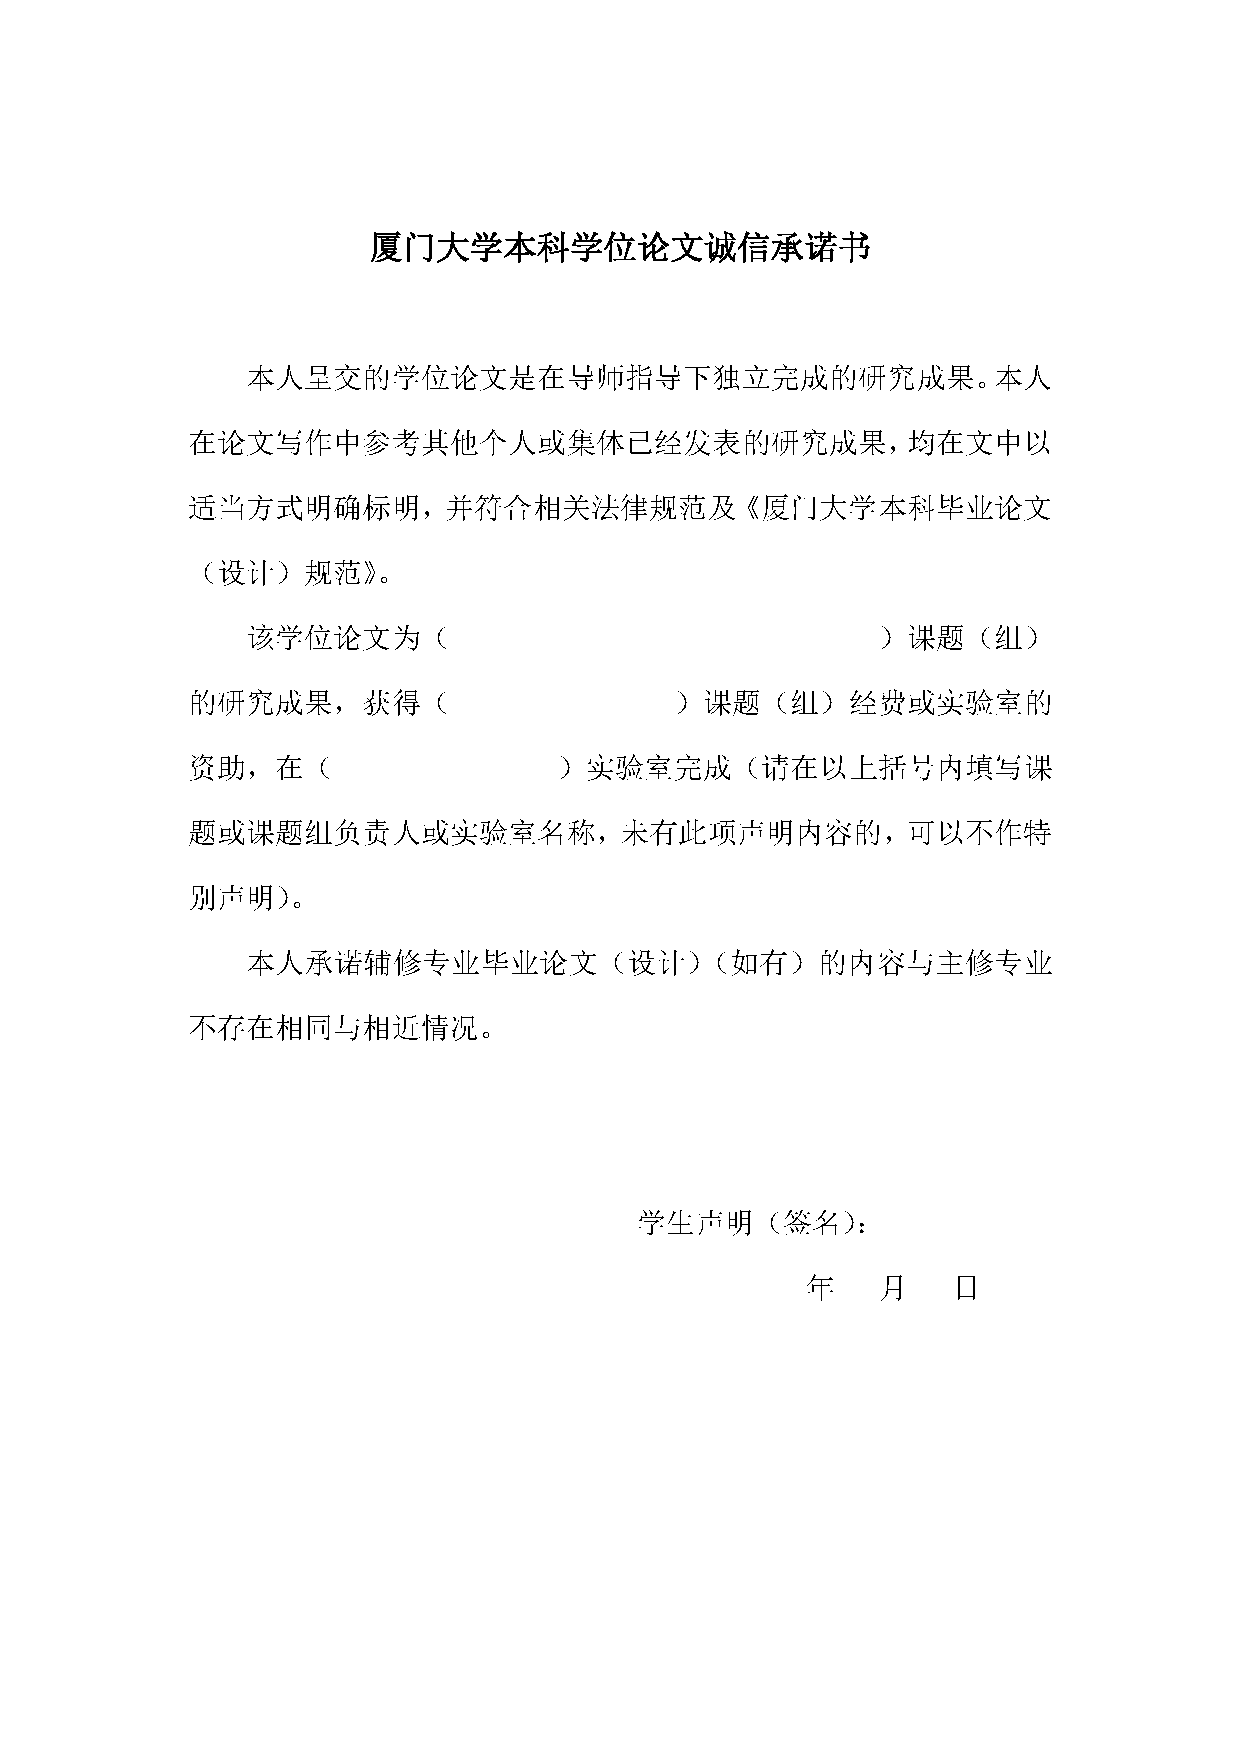
\includepdf[pages=-]{figures/promise.pdf}
  % 诚信承诺书原件,请修改内容后打印签名,扫描为 PDF 后添加
\clearpage
\begingroup
\pagenumbering{Roman}
\setcounter{page}{1}
\vspace*{1\baselineskip}

\begin{center}
  \XiaoSan \Song \bfseries 厦门大学本科学位论文诚信承诺书
\end{center}

\vspace*{1\baselineskip}

\SiHao \Song

本人呈交的学位论文是在导师指导下独立完成的研究成果。本人在论文写作中参考其他个人或集体已经发表的研究成果,均在文中以适当方式明确标明,并符合相关法律规范及《厦门大学本科毕业论文(设计)规范》。

% 自行填写
该学位论文为(\quad\quad\quad\quad\quad\quad)课题(组)的研究成果,获得(\quad\quad\quad\quad\quad\quad)课题(组)经费或实验室的资助,在(\quad\quad\quad\quad\quad\quad)实验室完成(请在以上括号内填写课题或课题组负责人或实验室名称,未有此项声明内容的,可以不作特别声明)。

本人承诺辅修专业毕业论文(设计)(如有)的内容与主修专业不存在相同与相近情况。

\vspace*{2\baselineskip}

\rightline{学生声明(签名):\quad\quad\quad\quad}

\rightline{\number\year 年 \number\month 月 \number\day 日}\hspace{2pt}
\endgroup

  % 致谢
  % 致谢
\begin{acknowledge}
  值此论文完成之际,谨向所有关心和支持我的人们致以诚挚的谢意!

  首先,我要衷心地感谢我的导师XXX教授。从论文选题、内容和整体结构的确定,直至最后定稿,XXX老师都以极其负责的态度给予悉心指导,为我提出了许多宝贵的意见和建议,使我获益良多。他渊博的学识、严谨的治学态度以及朴实的学术作风时刻激励我不断努力完善自己,对我的悉心关怀和教诲也将鼓舞我在今后的学习和工作上不断努力向上。在此,谨向XXX老师致以最诚挚的感谢!

  其次,还要感谢与我一起完成这个项目的所有团队成员。没有他们的帮助和共同努力,就没有项目的圆满成功,也就不会有本文的形成。在此,向他们表示衷心的感谢!
\end{acknowledge}

  % 摘要
  % 摘要(中文)

\xmusetup{
  keyword = 非结构化信息;信息可视化;可视分析
}

\begin{abstract}

随着信息的发展,出现了越来越多的非结构化信息。并且非结构化信息在政府和企业等的决策中扮演着重要的角色。如何将非结构化数据有效的管理起来,能够进行数据和知识挖掘,提取当中的隐含信息,提供一种形象的可视分析,为政府和企业决策提供支持成为当今亟待解决的主要问题。

本文以北京市科委的指数统计文档为研究对象,主要任务是针对以北京市科委的指数统计文档为代表的非结构化信息的抽取和企业指标信息的可视分析。主要工作包括三个方面:第一,设计了一套以北京市科委的指数统计文档编写规范为标准的确实可行的信息抽取算法;第二,针对抽取出来的指标信息,借助于Dundas可视化工具进行可视分析;第三,完成了一个满足客户需求的企业信息库管理系统。

论文从项目背景出发,介绍了系统开发的背景和研究价值。然后,详细介绍了企业指标信息智能处理的可行性和算法设计,以及企业指标信息可视分析的原理及其实现。再次,论文详细阐述了系统的需求,具体介绍了企业信息库管理系统的设计及其实现,最后论文针对企业信息库管理系统进行了分析和评价,并指明了下一步的改进计划。\footnote{这是一个注解示例。}

\end{abstract}
  % 英文摘要 (Abstract)

\xmusetup{
  en-keyword = Unstructured Information; Information Visualization; Visual Analysis
}

\begin{abstract-en}
With the development of information, there has been an increasing number of unstructured information. And it plays an important role in decision of government and enterprise, etc. How to manage the unstructured information efficiently, mine the data and knowledge, extract the implicit information, provide a visual image analysis, and then support the government and enterprise's decision have become the main issues to be settled urgently. 	

In this question for discussion, we mainly have a research in indicator of enterprise documents from the Beijing Science and Technology Commission and try to obtain the indicators of the unstructured information, and then provide a visual image analysis. It includes three aspects: First, to design a set of practical information extraction algorithm; second, through the use of the Dundas Chart toolbox, providing visual analysis; third, completed Enterprise Information Management System which meet customers requirement.

The beginning of the dissertation introduced the background of the project, introduced the background of the system and research value. Second, detailing information extraction algorithms and principles of Information Visualization. Third, the dissertation elaborated the system's requirement, specifically introduced the system design and implementation. Finally, some possible improvements and future works were presented.  
\end{abstract-en}

  % 目录
  \maketoc

  % 正文
  \beginbody
  \newchapter{绪论}{Introduction}

\newsection{引言}{Preface}

随着计算机技术的发展,使海量信息得以存在并迅猛发展。尤其是信息技术的日益普及其应用以后,随着各个行业的信息系统的规模的日益扩大,信息系统在长年累月的运转过程中,积累了庞大的数据资源。然而决策者却很难利用这些数据资源,为企业和政府的决策提供确实有效的帮助。这是因为一方面,在这庞大的数据资源中,非结构化信息占据了主要部分\cite{fsyang-skgao-1998}。 Gartner的一项调查显示,在今天的社会中,有80\% 以上的商业行为依赖于非结构化信息;我们所存储的数据中,85\%以上是非结构化信息;每过三个月,我们周围的非结构化信息就会增加一倍。这些数据充分说明,我们周围信息的形态是以非结构化信息为绝对主体的,也可以说我们接触到的信息中绝大部分是非结构化信息。因此对非结构化信息进行管理,能够进行数据和知识挖掘,提取当中的隐含信息,对决策进行支持成为当今亟待解决的主要问题 \cite{cbchen2008}。另一方面,随着信息技术的发展,信息结构越来越复杂,信息更新越来越快,信息规模越来越大,给人们获取信息、理解信息、掌握信息带来了沉重的负担,常常导致“认知过载”、“视而不见”\cite{dzzhang-ppzhang-2006}\cite{xdxie-1998}。

北京市科学技术委员会在企业指标信息统计分析工作上就存在这两方面的问题,文献\parencite{xdxie-1998}介绍了这方面的工作。每年北京市科委都要对北京市企业进行企业指标信息的调查,在长年累月的积累过程中,北京市科委积累了大量的企业指标调查表、项目立项、执行、验收等文档。这些调查表以word形式保存起来,并且调查指标的方式也呈现多样化,存在选择、填空、表格、问答以及这些题目的复合等形式。而且企业指标的调查涵盖范围也很广泛,从企业性质及登记情况到企业财务及信息化投入状况,再到人力状况及信息化支撑状况,到企业信息化基础设施建设状况、企业信息化应用情况,甚至涉及到企业对信息化工程的满意程度的调查。面对海量的非结构化企业指标信息,北京市科委每年都要投入大量的人力、物力、精力,将企业指标信息从word文档中手工提取出来,形成计算机可以识别的结构化的表格信息,再对企业指标信息进行统计分析。即使是这样,仍然存在许多问题:第一,手工抽取企业信息调查表耗时较长,工作强度大。第二,手工抽取数据信息容易出现错误,准确性不能得到有效保证,而且一旦出错,就有可能导致整个统计分析结果的错误,进行核对非常困难。第三,即使是将企业指标信息全部准确转成计算机可以识别的表格数据以后,由于数据的多样性,缺少形象的对企业指标信息的统计分析工具。 

针对北京市科委的企业指标信息统计分析问题,我的毕业设计结合北京市科委的业务需求,开发了企业信息库管理系统。这个项目来源于国家科技支撑计划项目课题“面向服务的智能化制造技术及示范应用”(课题编号2006BAF01A17)。该项目主要是为了解决北京市科委的指标信息统计分析过程中,存在指数统计困难和文档管理困难两个问题,以业务为主线,主要包括科委文档的管理、企业指标信息的智能处理、企业指标信息的可视分析三个方面的内容。通过为科委中存在的大量信息文档实体构建基础信息模型,来方便用户的日常管理和提高文档的利用率。通过构建应用数据模型,将企业指标信息文档中的非结构化信息智能抽取出来,并存储于数据库当中,将非结构化信息结构化,用成熟的结构化数据管理理论来管理非结构化数据。通过对指标信息的查询,构建信息可视分析模型,使用户可以对知识进行挖掘,提供形象的可视分析,提高北京市科委的企业指标信息的统计分析效率。本项目完成后将会在北京市科委投入使用。

\newsection{论文组织结构}{Organization of Thesis}

本论文共分为六章,论文首先分析了政府和企业在信息化过程中遇到的两个问题:非结构化信息管理和“认知过载”。并结合北京市科委的企业指标统计分析问题,介绍了毕业设计项目的背景和研究价值,引出了论文所做的主要工作内容。紧接着论文简单概述了毕业设计项目中所用到的各项技术,并针对北京市科委的业务要求提出了信息抽取和基于Dundas Chart信息可视化的解决方案。然后论文就项目中的两个技术难点——非结构化信息处理和信息可视分析,详细阐述了信息抽取技术的算法设计和信息可视分析技术的模型设计。在系统实现方面,论文详细介绍了企业信息库管理系统所使用的技术要点:基于Asp.net的三层结构(USL-BLL-DAL)的框架设计;在用户体验方面,采用了Asp.net Ajax改善用户的体验 \cite{ll-soidc}。

论文具体安排如下:

第一章\ 简单介绍了企业和政府在信息化过程中遇到的非结构化信息管理困难和“认知过载”问题。针对北京市科委的指标统计分析问题,提出了毕业设计的背景、目标和研究价值。

第二章\ 概述系统中所使用的各项技术及各项技术的国内外发展现状。

第三章\ 详细介绍了针对北京市科委企业指标信息文档的信息抽取技术的算法设计和信息可视分析的模型设计。

第四章\ 介绍了企业信息库管理系统的实现。详细阐述了系统的背景和总体目标,基于表示层(USL)-业务逻辑层(BLL)-数据访问层(DAL)的三层结构的框架设计和功能模块介绍及其实现。

第五章\ 介绍了企业信息库管理系统的系统测试和运行结果。

第六章\ 最后论文总结了毕业设计所做的工作,并且指明了下一步的改进计划。主要是在信息抽取算法的改进,以及在用户体验方面的改进计划。

  \newchapter{系统相关技术概述}{System Related Technologies Outline}
  
\newsection{非结构化信息处理}{Unstructed Information Management}

\newsubsection{非结构化信息管理概述}{Introduction of Unstructed Information Management}

在引言中,我们提到过“在当今的社会中,我们周围信息的形态是以非结构化信息为绝对主体的, 也可以说我们接触到的信息中绝大部分是非结构化信息。”,那么什么是非结构化信息?非结构化信息具有什么特点?如何管理非结构化信息?

信息可以分为三类:结构化信息,非结构化信息和半结构化信息。

\begin{enumerate}[topsep=0pt]
  \item [1、] 结构化信息——经过严格标引后的数据,一般以二维表的形式存在。如数据库中的表、各种票据信息等等。\\ 结构化信息又分为以下三种:
  \begin{enumerate}[topsep=0pt]
    \item [(1)] 一维结构化信息。\\ 一维结构化信息可以进一步分为以下两类:
    \begin{enumerate}[topsep=0pt]
      \item [(a)] 第一类一维结构化信息。
      \item [(b)] 第二类一维结构化信息。
    \end{enumerate}
    \item [(2)]二维结构化信息。
    \item [(3)]三维结构化信息。
  \end{enumerate}
  \item [2、] 非结构化信息——没有经过人为处理的不规整的信息。这些信息更加符合人类交流的方式。如新闻报道、科技文献、散文等等。
  \item [3、] 半结构化信息——介于结构化信息和非结构化信息之间的。有一定格式约束,这不同于非结构化信息,但局部上,又按人类自然语法组织信息,与结构化信息又有所区别,例如电报报文,通知、公告、指数统计表等等。
\end{enumerate}

非结构化信息具有如下特点:第一,其格式非常多样;第二,标准是多样性的,不像我们结构化的数据一目了然;第三,在技术上非结构化信息比结构化信息更难标准化和理解。所以存储、检索、发布以及利用需要更加智能化的计算机技术。

基于非结构化信息的特点,将非结构化信息结构化,转化为结构化信息进行管理是一个可行的管理方案,而构建的面向用户的企业非结构化信息管理系统必须具备以下特征:

\begin{enumerate}[topsep=0pt]
  \item [1、] 必须对非结构化信息资源的获取、转换、分析、管理、应用全过程进行分析,提供基于标准工作过程的支持环境。
  \item [2、] 必须提供标准的对外接口、信息描述方法和定制规范降低定制分析机组件和信息应用组件的复杂性。
  \item [3、] 必须提供灵活的信息描述资源模式简化信息结构化信息资源库的构建。
  \item [4、] 采用自然资源技术以支持高质量的“拉式”信息服务和知识抽取。
  \item [5、] 提供对外的标准的接口以支持非结构化信息资源管理系统与企业其他应用系统的集成。
  \item [6、] 提供界面友好的工具方便用户系统管理和应用。
  \item [7、] 其本身应具有易于扩充、动态发展的能力。
\end{enumerate}

图 2-1 为基于UIMA(Unstructured Information Management Architecture)的非结构化信息管理的架构图,具有一定的指导意义:

\begin{newfigure}
  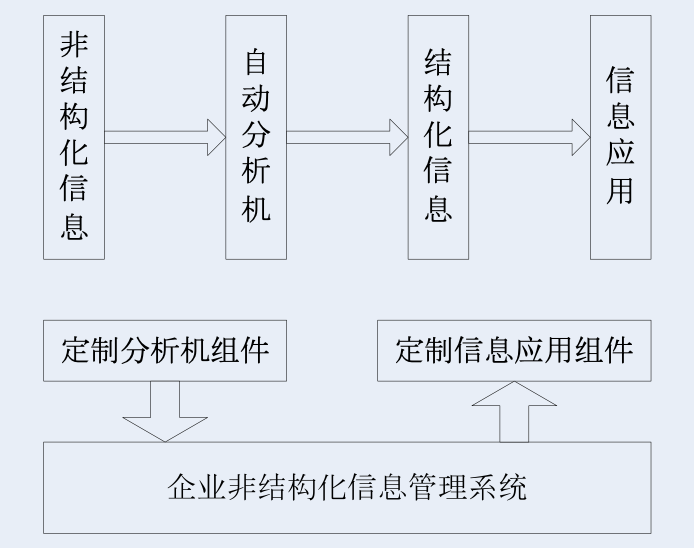
\includegraphics[width=0.3\paperwidth]{figures/figure1.png}
  \caption{企业非结构化信息管理系统应用模式\cite{xdxie-1998}}
\end{newfigure}

在把列名映射到Dundas里面的图例,而行名则映射为Dundas里的轴标签。完成了数据表的映射以后,剩下的就是图表自身形态的改变了。为了实现Dundas形态的改变,我们对Dundas的属性进行了分类和总结,如表2-1所示:

\begin{newtable}
  \caption{Dundas的部分属性表}
  \begin{tabular}{ll}
    \toprule
    属性 & 描述 \\
    \midrule
    图表类型(Chart Type) &	条柱型图表(Bar and Column Charts):条形图、柱状图;\\[2ex]
    线型图表(Line Charts) & 折线图、曲线图、阶梯图;\\[2ex]
    点图表(Point Charts) & 点图、泡泡图;\\[2ex]
    饼图(Pie Charts) & 饼图、圈图;\\[2ex]
    分区图(Area Charts) & 折线分区图、曲线分区图;\\[2ex]
    条柱宽度 (Point Width) &	针对条柱型图表,条柱的宽度。取值从(0,1)。\\[2ex]
    条柱风格 &	针对条柱型图表,有默认、砖型、圆形、棱型、明暗变化\\[2ex]
    数值标签 (Value Label)	& 是否显示数值标签。\\[2ex]
    3D显示	& 是否3D显示。\\[2ex]
    簇状显示 &	是否簇状显示。\\[2ex]
    图例 (Legend) &	字体属性;字号属性;显示位置:图表的左边、右边、上面、下面。\\[2ex]
    标签(Axis) &	字体属性;字号属性。\\[2ex]
    标题(Title) &	字体属性;字号属性。\\[2ex]
    \bottomrule
  \end{tabular}
\end{newtable}

选择算子决定了哪些染色体进入下一代。本算法中采用“轮盘赌”的选择方式,它按照染色体的适应值大小来确定该染色体的被选择概率。如果染色体的适应值越大,其被选中的概率越大。个体 $r_i$ 被选中的概率 $p(r_i)$ 定义如下:

\begin{align}
p(r_i) = Fitness(c_i) / \sum_{j=1}^{pSize} Fitness (c_j), (pSize \mbox{为种群大小}) \tag{公式 2-1}
\end{align}

确定了每个染色体的被选择概率后,系统生成一个在 $[0,1]$ 区间的随机数组,然后与对应染色体的被选择概率比较,如果随机数大于染色体的被选择概率则该染色体被选择,反之被淘汰。

\begin{definition}
如果存在一条从 $V_i$ 到 $V_j$ 的路,称 $V_i$ 是 $V_j$ 的前驱节点,而对于 $(V_i, V_j) \in E$,称 $V_i$ 是 $V_j$ 的立即前驱节点,记为$Vi \in iPred(V_j)$,称 $V_j$ 是 $V_i$ 的立即后继节点,记为 $V_j \in iSucc(Vi)$。
\end{definition}

定义一个公共容器类型的代码如下:

\begin{minted}{c++}
class Container : public Object{
public:
  virtual Object* get();               // 删除并返回当前元素
  virtual void put(Object*);           // 在当前元素之前插入
  virtual Object*& operator[] (size_t);  // 下标
  //…
};
\end{minted}


  % 参考文献
  \makerefs

  % 附录
  \makeappendix
\end{document}